

%  d) shows a step by step process when using AIv2. For a, b, and c, 1, 3, 5, 9, 11, relate to participants 1, 2, 3, 5, and 6, respectively.

\begin{figure*}[h!]
 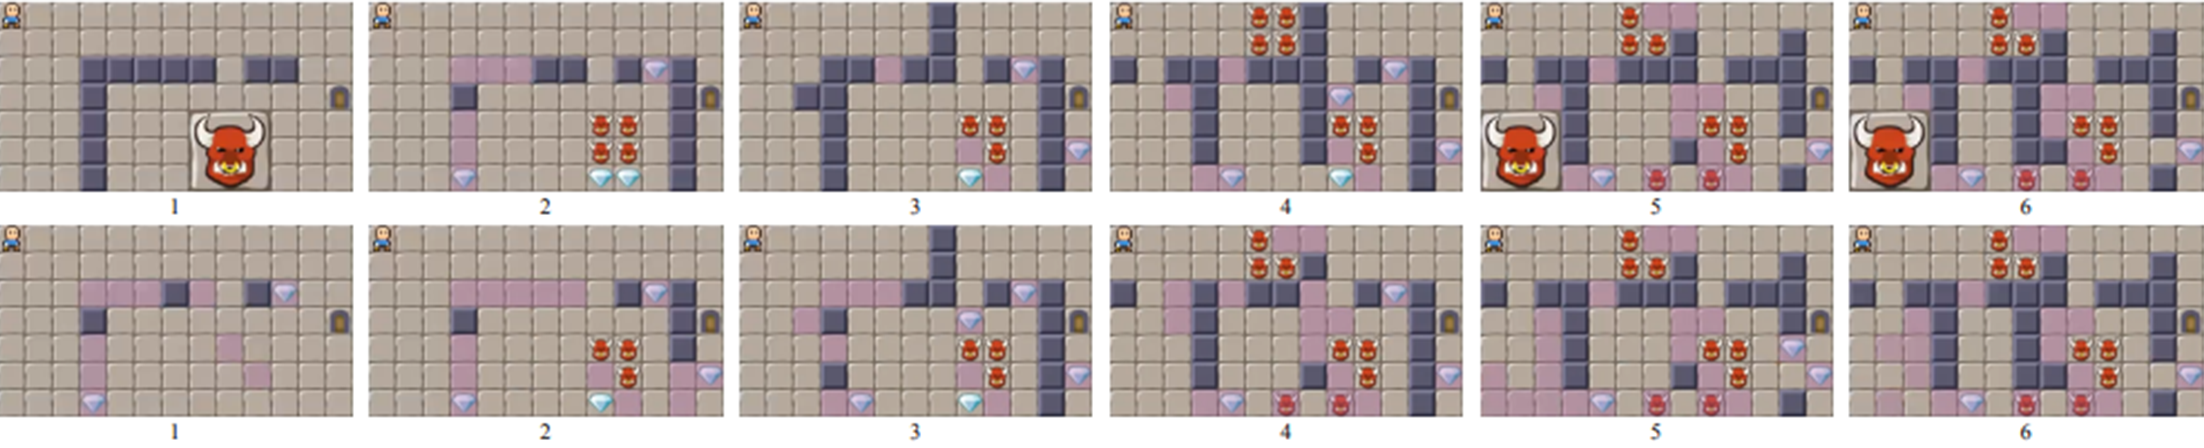
\includegraphics[width=\textwidth]{images/rooms-designed-2.png}
 \caption{Sample step by step process when using AIv2. Human's turn is top row, while the AI's turn is the bottom row.}
 \label{fig:exampleDesignProcess}
\end{figure*}

\subsection{Discussion}
\label{sec:discussion}
% This section contains an analysis of the results presented in Section VI, as well as a discussion to connect the results to the theoretical framework and the specific aspects relating to the research questions. 


\subsubsection{Willingness to include the AI in the design process}

All participants expressed an interest and willingness to see what the AI could come up with to design the rooms, emphasizing that they either considered or incorporated the ideas brought forward by the AI, which further supports other MI-CC research conclusions~\cite{p13guzdial_friend_2019,bhaumik_lode_2021}. However, many participants expressed multiple frustrating factors, and based on figure~\ref{fig:human-ai-contribution}.a, when given the opportunity, the human designers did not include much of the AI's contribution but might have provided some ideas that either influenced or were part of the final design. Figure~\ref{fig:human-ai-contribution} also displays that as the AI got more agency, the AI tiles at the end design increased. This can be due to frustration expressed by participants where they didn't agree with the AI design and ended up handing over the control to the AI and giving up, to some extent, their aspiration to create. The lower meso- and spatial-patterns combined with the lower symmetry in AIv3 are also part of the issue. The fewer patterns that exist mean that the rooms are less structured, which, combined with no way to correct these, could result in designers feeling that the levels are more ``random".


%in general, this would make designers less 

 %as th, except for Symmetry, which reduces as the AI gains more agency. Similarly, patterns are reduced when using high agency, which shows  

%As expected, the amount of tiles remaining at the end design increased as the AI got more initiative.


%All of the participants expressed an interest and willingness to see what the AI could come up with. Many of the participants expressed that they either considered the ideas brought forward by the AI, or incorporated them. This further strengthens the conclusion made in other studies exploring MI-CC Game Design tools, that human designers are interested and willing to using MI-CC to create game content. However, as many of the participants also expressed multiple frustrating factors when using the tool,Additionally, the quantitative data further suggests that when proposed with the option, many of the human designers where in fact not including a lot of the AI's contributions in their end products.


%As displayed in Figure 6 with the resulting rooms, and Figure 9 with the representation of tiles in the resulting rooms, the human designers where disinclined to incorporate the AI-placed tiles in the final product when using AIv1. As displayed in Figure 9, the human designers generally did not place down many of the suggestions that the AI made in AIv1. This suggests that the version of the AI with low initiative did not have great influence on the final design, however the AI might have provided some ideas that either influenced or was part of the end product.
%When comparing Figure 12, 13 and 14, displaying the divisions between the tiles in the resulting rooms, one the general pattern can be identified, namely, as the AI gains initiative, the AI has an increasing impact on the final product. As many participants expressed that the AI made creations that they did not agree with, and that they handed over the control to the AI and gave up their aspiration to create, the end product consisting of a majority AI-placed tiles is likely because of this frustration. 



\subsubsection{Variants of the users}

Most participants used the tool similarly except for participants 1 and 6. Participant 1 didn't want to incorporate the AI's contributions, as it can be seen in fig.~\ref{fig:human-ai-contribution}, explicitly stating that ``... I don't think level design is a good place for an AI that has more control than the human... The little details that I love in level design would never be created by an AI. Nice little references, or easter-eggs, or how humans get inspired by simple things..." On the other hand, participant 6 recurrently incorporated many of the AI's tiles. When using AIv2 and AIv3, they pressed ``End Turn" repeatedly to find out what the AI would be able to create, commenting ``I want to see if it can create something cool." However, while their approach was completely different, they both agreed that they would prefer the AI to create a complete room, and they could polish it from there.

% , which is the common approach in MI-CC~\cite{p13sentient-sketchbook,eddy1}.

%Out of the eight participants there were two in particular, who used the tool in very different ways from each other. Participant 1, who created room 1 and 2, had a strong inclination to not incorporate the AI's contributions. This is suggested in Figure 12 and Figure 13, where the final product consisted of over 95\% human-placed tiles when using AIv1 and AIv2, as seen as bar 1 and 2 in both charts.
%Participant 1 is a professional game designer, and has 8 years of professional experience within the field. They expressed the following:

%\textit{"I only see the usage of the Medium and High in the purpose of typical PCG-tools, like populating areas fast and efficiently. I don't think level design is a good place for an AI that has more control than the human. I think there are other areas where it fits better, such as PCG, creating big arrays of content where randomness is something you want, enemy clusters et cetera." ... "The little details that I love in level design would never be created by an AI. Nice little references, or easter-eggs, or how humans get inspired by simple things like walking in London and seeing a cool building, you want to put that into a level. I think AI can handle high-level stuff, like compositions of shapes and light and stuff, but that the details should be left to the human."}


%Participant 6, a third year Game Development-student, who created room 11 and 12, included a lot of the AI-placed tiles in their final products when using AIv2 and AIv3, as displayed in Figure 13 and Figure 14. Room 11 with AIv2, as shown as bar 11 in Figure 13, was the only room where all tiles placed in the end product where AI-placed tiles. This is also shown in Figure 7, as Room 11. Multiple times while using AIv2 and AIv3, Participant 6 pressed "End Turn" repeatedly, to find out what the AI would create. One of those times, the participant commented: 

%\textit{"I want to see if it can create something cool." }


%In the interview, when answering Question 11, Participant 6 suggested that a possible improvement to the tool could be displaying complete generated rooms, which the human can choose from and then edit a set amount of tiles in. This suggestion is very similar to the original state of EDD, which was used to modify for this project, works.  
%Interestingly, despite the differences in how  Participant 1 and Participant 6 used the tool, the way Participant 1 described their opinions of a better use of the tool, as an efficient way to generate rooms with the human polishing some final touches, is similar to how Participant 6 actually used the tool. 
%Additionally, as Participant 6 expressed interest in a tool similar to the original state of EDD, to efficiently create rooms with minor influence from the human, however control in the form of selecting out of the generated rooms, and polishing the rooms, this also coincides with the opinions of Participant 1.


\subsubsection{Frustrating factors and Constraints}

% When using EDD, the participants expressed multiple frustrating factors.
The participants expressed multiple frustrating factors within the tool. The main point was the repetitive behavior of overwriting the human tiles with floor tiles, removing their ideas without contributing with anything of value, and the human designer feeling forced to move on from those positions and contribute somewhere else in the room. This was exacerbated when using AIv2 as, unlike AIv1, the AI placed down the tiles rather than suggesting, and unlike AIv3, the human designer still had the option to overwrite the AI-placed tiles. The human designers assign value to each tile type as they provide different aspects in level design; for instance, participants often placed enemies and treasures close to each other, possibly to create a risk and reward in the level. Figure~\ref{fig:exampleDesignProcess} shows one example of a participant creating a room using AIv2, step by step. The human designer's first contribution includes a long continuous wall and a boss. When the AI has its first turn, it contributes with floor tiles overwriting the designer's tiles. Towards the end of the design, the human designer places a boss tile in the bottom left corner that the AI overwrites with floor tiles twice before the human designer gives up and finishes the room without a boss. This sample creation process shows that the AI tried to steer the room towards more leniency and open areas, which contradicted the human's goal. 

Another main frustrating factor was the loss of control experienced by human designers when co-creating with the AI, especially AIv3. Participants expressed that the AI's decisions limited them and were forced to work around what the AI designed. As the AI gained control, they felt their creative process got increasingly constrained. This aligns with the Lode Encoder study~\cite{p13bhaumik_lode_2021}, where the participants expressed frustrations with completing a playable level, as they were forced to rely on the AI to generate the option they wanted in the final stages of the level creation. Further, when using AIv3, the number of positions that the human has available decreases with every turn, while the AI can continue to place tiles on any position, which unavoidably limits the human's control over the final design.

Most of the participants felt frustrated and constrained as the AI gained more control over the design process. Additionally, all participants suggested removing the turns and constraints of the number of tiles per turn to improve the tool. Three of the eight participants expressed that adjusting the AI's role to one of an assistant to the human designer would improve their creative experience. 

%A few of the designers expressed a dislike of the turn-based creative process, as well as the constraint of maximum amount of tiles per turn. These participants expressed that they felt they were not collaborating with the AI, but rather working against each other and fighting for control over the design.  

%The participants expressed a dislike of the constraining nature of AIv3, where they are limited by the AI’s decisions, and that they were forced to work around what the AI designed. In the study of the MI-CC tool Lode Encoder, by Bhaumik et. al, the human designers where constrained to only use the content that the AI generated~\cite{p13lode-encoder}. The participants in the study of Lode Encoder expressed frustrations with completing a playable level, as they where forced to rely on the AI to generate the option they wanted in the final stages of the level creation. The increasing frustration some participants felt as the level creation proceeded when using Lode Encoder, is notably similar to the increasing frustrations the participants of this study expressed when using AIv3. The participants grew discontented as they where increasingly constrained by the AI's creations.


%When using AIv3, one particular constraint is very present. As the amount of positions that the human can place new tiles in decreases with every turn, while the AI can continue to place tiles on any position, there is an unavoidable limitation for the human designer. Many of the participants found this version of AI and this constraint particularly frustrating, and expressed that they gave up and let the AI control the design after few turns. This also is supported by the data, displayed in Figure 14, which shows that the resulting rooms from using AIv3 generally consisted of a majority of tiles placed by the AI. 




%The participants expressed multiple frustrating factors within the tool. One of the most commonly mentioned factor occurred when using AIv2. Many participants experienced that the AI used its turn to overwrite the walls, treasures, enemies and boss-tiles the human just placed down with floor-tiles. 

%When using AIv2, this behaviour in the AI was the most prevalent, as unlike AIv1, the AI placed down tiles during its round outside of the human designers control, and unlike AIv3, the human designer still had the option to overwrite the AI-placed tiles. In this version of the AI, this often created a frustrating back and forth for the human designers, where the AI spend its turn "removing" what the human designer had just placed, and the human designer spends their following turn replacing the same tiles again. This often was repeated until the human designer gave up, or the MAP-elites algorithm had finished a new run and the AI made different decisions.


% \begin{figure*}[h]
%     \centering
%     \includegraphics[width=\textwidth]{images/steps.png}
%     \caption{Step by step process of one participant using AIv2 to create a room. The top row shows what the human contributed with during the human's turn, the bottom row display what the AI responded with during its turn.}
%     \label{fig:my_label}
% \end{figure*}

%Figure 20 shows one example of a participant, Participant 5 creating his first room using AIv2, step by step. The human designer's first contribution includes a long continuous wall, as well as a boss-tile. When the AI has its first turn it contributes with floor tiles overwriting the long wall, and the boss tile. Towards the end of the design, the human designer places a boss tile in the left bottom corner, that the AI overwrites with floor tiles twice, before the human designer gives up and exits the room editing view without a boss in the room.


%The participants perceived the AI's seeming preference of overwriting human-placed tiles with floor-tiles as the AI removing their ideas, without contributing with anything of value. This suggests that human designers assign a value to each type of tile, as they provide different aspects of game level design. For example, participants seemed to value boss-tiles highly, as they provide a big challenge. The participants often placed enemies and treasures close to each other, possibly to create a risk and reward in the level. The AI however, does not value the tiles this way, and therefore is more prone to placing floor-tiles than the human designer is.
%As displayed in Figure 18, the most common types of tile to place as a human designer in descending order is wall, treasure, enemy, floor and finally boss. Comparing this data to the AI-placed tiles, displayed in Figure 19, the AI is considerably more prone to placing floor tiles, as it is the most common type of tile placed by the AI.
%As only 5\% of tiles placed by human designers where floor-tiles, compared to 61\% of the tiles placed by AI, the perception of an AI-agent with a fondness of overwriting human-placed tiles with floor-tiles is very likely accurate.


%Another notable difference in the tiles that the different co-creators placed is that the AI never placed a boss tile.  Moreover, many participants expressed that the AI placed floor-tiles where they had placed a boss-tile, actively removing the boss. As shown in Figure 6, 7 and 8, many of the participants where prone to creating one normal room as their first room, and secondly one boss-room, for each version of the AI. Also displayed in Figure 6, 7 and 8, is the pattern that the amount of boss-tiles in the resulting rooms decreased with an increase of initiative from the AI. This further correlates with the notable disagreement between AI and human designers in terms of valuing tiles differently, and how it affected boss-tiles in particular. 


%One other main frustrating factor that was brought up was the loss of control that the human designers experienced when co-creating with the AI with high initiative, AIv3. This was many of the participants motivation to name AIv3 as the version they liked the least. The participants expressed a dislike of the constraining nature of AIv3, where they are limited by the AI’s decisions, and that they were forced to work around what the AI designed. In the study of the MI-CC tool Lode Encoder, by Bhaumik et. al, the human designers where constrained to only use the content that the AI generated~\cite{p13lode-encoder}. The participants in the study of Lode Encoder expressed frustrations with completing a playable level, as they where forced to rely on the AI to generate the option they wanted in the final stages of the level creation. The increasing frustration some participants felt as the level creation proceeded when using Lode Encoder, is notably similar to the increasing frustrations the participants of this study expressed when using AIv3. The participants grew discontented as they where increasingly constrained by the AI's creations.

%\subsubsection{Constraints}

%Many of the participants expressed that as the AI gained control, they felt increasingly constrained in their creative process. When using AIv2, some participants felt constrained when the AI repeatedly overrode human-placed tiles with floor, and the human designer felt forced to move on from those positions and contribute somewhere else in the room. Another constraint that arose from this behaviour in the AI, was that many participants expressed that the AI did not allow them to place boss-tiles, and the human designer therefore was constrained to not create a boss room, as they had initially had intended. 


%When using AIv3, one particular constraint is very present. As the amount of positions that the human can place new tiles in decreases with every turn, while the AI can continue to place tiles on any position, there is an unavoidable limitation for the human designer. Many of the participants found this version of AI and this constraint particularly frustrating, and expressed that they gave up and let the AI control the design after few turns. This also is supported by the data, displayed in Figure 14, which shows that the resulting rooms from using AIv3 generally consisted of a majority of tiles placed by the AI. 


%A few of the designers expressed a dislike of the turn-based creative process, as well as the constraint of maximum amount of tiles per turn. These participants expressed that they felt they were not collaborating with the AI, but rather working against each other and fighting for control over the design.  



\subsubsection{The concept of a well performing, high agency co-creator}

%Since there is a willingness from human designers to incorporate AI into creative processes, and there exist distinct advantages of using MI-CC, it is important to identify why this tool did not provide a satisfactory creative experience. 



Most participants showed a willingness to incorporate AI into the creative process, contributing with new ideas or performing services such as ensuring feasibility. Yet they were reluctant to incorporate higher agency AI, which suggests that the AI needs to be aligned with their goals, intentions, and procedures, i.e., have an accurate designer model~\cite{p13liapis_designer_2013}. Within EDD and level design tools, multiple practical improvements are to be made. Five participants described the AI's behavior as random and unpredictable, especially when overwriting human-made structures and contributions. The AI currently calculates the most common tiles in the positions of the contribution area and contributes with the tiles of highest occurrence among a set of generated elites. This contradicts how human designers perceive the design importance of tiles, valuing higher usable tiles rather than floors. The AI could then weigh higher those and the combined structures they create. Additionally, the AI could favor unedited areas before overriding human-placed tiles to support rather than override. 

Another important point is that all AI versions are static in the design process, which means that the AI follows the same procedure regardless of the agency level. The collaboration do change in the design process (e.g., suggest or directly placing tiles, or if AI tiles can be removed) but other aspects and parameters do not change or adapt to designers. These parameters are connected to the overarching design of the AI rather than the AI's agency, which might have affected the designers' perception. For instance, given that the AIv3 tiles could not be replaced, changing the amount of tiles, rectangular area, or its adaptability in regards to what the designer had created thus far could be beneficial.

%Adaptation could take place by using designer modeling to tailor the changes. We could also analyze the designers' trajectory in relation to the behavioral dimensions. Then, we could map how the room has changed regarding the dimensions and what type of goal the designer might be going towards, and bias the KNN distance metric towards that.

%We could also or by analyzing the designer' current trajectory in the behavior space. Their trajectory in relation to the behavioral dimensions, we could map how the room has changed regarding the dimensions and what type of goal the designer might be going towards. Then, KNN could bias the neighborhood towards those.

%The AI does collaborate differently in the design process (e.g., how to place tiles or 

Furthermore, the AI seemed to break apart walls and open up sub-rooms. This is possibly a result of the Linearity and Meso-Pattern dimensions in the MAP-Elites algorithm. The resulting elites of the generated rooms with the highest linearity will have the highest amount of traceable paths. Many participants seemed to want to create rooms with long walls, sub-rooms, paths that required the player to encounter enemies, and common aesthetical features such as symmetry. Analyzing the path designers are taking in these dimensions could better inform the search for content and the generation of elites, so the content is adapted to those preferences. However, adapting these dimensions might be counterproductive for the other dimensions, as symmetric rooms might not create balanced rooms regarding the Leniency dimension as it might not be considered as important. Another approach could be to incorporate designer modeling. By identifying possible design goals or design styles of the human co-creator, the AI can adjust its decisions and behavior to offer different levels of support depending on the human designer's behavior~\cite{p13liapis_designer_2013,alvarez_designer_2022}. 

%Furthermore, the AI seemed to break apart walls and open up sub-rooms. This is possibly a result of the Linearity and Meso-Pattern dimensions in the MAP-Elites algorithm. The resulting elites of the generated rooms with the highest linearity will have the highest amount of traceable paths. Many participants seemed to want to create rooms of low linearity, with long walls, sub-rooms, and paths that required the player to encounter enemies. Likewise, symmetry was sought by most designers, which is a common aesthetical feature. Analyzing the path designers are taking in these dimensions could better inform the search for content and the generation of elites, so the content is adapted to those preferences. However, adapting these dimensions might be counterproductive for the other dimensions, as symmetric rooms might not create balanced rooms regarding the Leniency dimension as it might not be considered as important. Another approach could be to incorporate designer modeling. By identifying possible design goals or design styles of the human co-creator, the AI can adjust its decisions and behavior to offer different kinds of levels of support depending on the human designer's behavior~\cite{p13liapis_designer_2013,alvarez_designer_2022}. 



%The majority of the participants preferred the version of the AI with low initiative, AIv1. The second most preferred version of AI was AIv2. However, as there is a willingness from human designers to incorporate AI into creative processes, and there are distinct advantages to use MI-CC in game level design, it is important to identify why this tool did not provide a satisfactory creative experience, as well as how this can be used in further research to allow our understanding and development of MI-CC to be further developed.

%A majority of the participants felt frustrated and constrained as the AI gained more control over the design process. Additionally, all participants suggested removing the turns and constraints of amount of tiles per turn to improve the tool. Three of the eight participants expressed that adjusting the AI's role to one of an assistant to the human designer would improve their creative experience. Although a willingness to incorporate an AI agent who displays new ideas, or performs services such as ensuring feasibility has been identified among the majority of the participants, they are seemingly more reluctant to incorporate an AI of higher initiative and influence into their creative process. This suggests that for human designers to have a satisfactory experience with a MI-CC tool with an AI of high initiative and definitive impact on the design, the AI must achieve a level of behaviour which the human agrees with.


%As this study explicitly aimed towards exploring the limitations and possibilities of a MI-CC-tool with an AI with high initiative and definitive impact on the creations, it is of importance to attempt to identify possible solutions to this problem. To develop an artificially intelligent co-creator who performs well, possibly human-like, makes valuable and satisfactory decisions that the human designer appreciate and wants to incorporate, is arguably a challenging task.


%However, within the scope of EDD and this specific study, there are multiple possible improvements to be made.
%Many of the participants, five out of eight, described the behaviour of the AI as random and unpredictable. One of the issues with the behaviour of the AI, as expressed by the participants, is its proneness to override walls, treasures, enemies and bosses with floor-tiles, especially human-placed tiles of these types.
%One possible improvement of this is to rework the choice of tiles to contribute within the AI-component. The AI currently calculates the most common tiles in the positions of the contribution area, and contributes with the tiles of highest occurrence. As previously discussed, this contradicts how the human designers view the tiles and their importance in the room, as humans seem to value bosses, enemies or treasures higher than floors or walls. By adjusting this part of the AI to not equate all tiles as being of the same importance in the design, but rather favoring to change floors over bosses for example, the AI could possibly behave more human-like.
%Additionally, the AI could favor to place tiles on top of untouched positions before overriding the human-placed tiles, to further support the human's creation before suggesting changes.


% Furthermore, some participants expressed that the AI placed floor tiles on top of wall tiles, seemingly to break apart longer walls and open up sub-rooms. This is possibly a result of the dimensions linearity and meso-patterns in the MAP-elites. The resulting elites of the generated rooms with the highest linearity will have the highest amount of traceable paths. Many participants seemed to want create rooms of low linearity, with long walls, sub-rooms, and paths which required the player to encounter enemies. One other notable possible preference among the participants was a seeming attraction to symmetry (See Figure 6, 7 and 8). Human attraction to symmetry is very common, and the fact that many designers seem to aim towards creating symmetric rooms is not unexpected. The dimension representing symmetry in the MAP-elites is valued equally to the other dimensions, which contradicts the suggested human favoring of this particular attribute.

% By adjusting the importance or influence of the different dimensions, the AI will contribute according to these preferences. For example, by valuing symmetry as ten times as important as all other dimensions, the AI would very likely only create symmetric rooms, however will likely not create balanced rooms as the leniency-dimension would not be considered as significant. To adjust the importance of specific dimensions in an effort to improve the AI, one would have to experiment and evaluate how to adjust these variables to create the most well-performing and human-like agent.
% Liapis et. al. performed research related to this idea, by exploring the adaptation of visual aesthetics depending on the user, with the help of AI~\cite{p13adapting-models-visual-aesth}. In their study, the explored how 2D spaceships could be generated by ML-PCG according to the user's tastes and preferences, and how humans valued the different aesthetic attributes. The study concluded that this could be a valuable strategy to create visually satisfying content through AI, for varying types of human designers~\cite{p13adapting-models-visual-aesth}.


% Another example of how the AI could be improved to make more human-like and predictable decisions is by reworking the AI to incorporate designer modelling. By identifying possible design goals or design styles of the human co-creator, the AI can adjust their decisions and behaviour to offer different kinds, or levels of, support depending on the human designer's behaviour. As the study performed by Alvarez et. al. discussed, this area requires more research, however shows great promise as a way to develop well performing AI in MI-CC tool~\cite{p13designer-modelling}. As of now, Alvarez et. al. are currently working on implementing and evaluating designer modelling in EDD. When it is implemented, it will likely be a relatively easy incorporated improvement to the AI of this version of EDD.












